\chapter{Tecnologie utilizzate}                 
\fancyhead[RO]{\bfseries Tecnologie utilizzate} 

Portare il 3d nel web non è cosa di poco conto. In un continuo processo evolutivo, gli sforzi di molte aziende ed utenti si sono sommati fino a creare il complesso ecosistema di tecnologie che oggi ci consentono di avere un pizzico di virtualità all'interno del browser. Nel seguito vengono illustrati uno ad uno questi strumenti, in ordine di apparizione, per avere una visione d'insieme chiara e completa. Alcuni di questi sono stati creati e sono evoluti pensando al web. Altri sono stati riadattati per essere integrati nel browser e per interagire con il World Wide Web.
 
Le tecnologie trattate di seguito sono tutti standard aperti\footnote{Open Inventor. (2011, July 12). In \textit{Wikipedia, The Free Encyclopedia}. Retrieved 09:05, August 25, 2011, from \url{http://en.wikipedia.org/w/index.php?title=Open_Inventor&oldid=439077866}}, le cui specifiche sono disponibili pubblicamente e gratuitamente e chiunque può contribuire al processo di decisione e di sviluppo. Questo lavoro non può e non vuole considerare soluzioni chiuse e proprietarie.

\clearpage
\section{Extensible 3D Markup Language}
In principio era VRML. Il Virtual Reality Modeling Language nasce nel 1994 e viene ratificato come standard ISO nel 1997 con il nome VRML97\footnote{ISO/IEC 14772-1:1997 – Per maggiori informazioni si veda \url{http://www.web3d.org/x3d/specifications/vrml/}}. Questo linguaggio consente di rappresentare una scena 3d in un semplice file di testo con estensione “wrl”, detto anche “world”. Vertici, spigoli, materiali, parametri per il texturing ed effetti, gestione luci, animazioni e suoni sono specificati in una struttura ad albero di tipo “scene graph” con una sintassi\footnote{La sintassi di un file VRML si basa sul formato standard Open Inventor, prodotto da SGI} semplice ed intuitiva. Grazie a nodi sensore ed eventi è gestita l'interazione con l'utente. Si possono inoltre inserire degli script, codificati in java o javascript, in dei nodi appositi, garantendo la massima flessibilità ed adattabilità della scena disegnata.

Come in ogni nuovo standard, vi erano in VRML delle evidenti lacune che andavano colmate. Una delle maggiori critiche sollevate da utenti e sviluppatori era la mancanza di una naturale integrazione con HTML. Per dirlo con le parole di Chris Phillips, sviluppatore per uno standard concorrente di VRML conosciuto come Chromeffects, \textit{``VRML has no integration with HTML. When the VRML guys built VRML [...] it was all about 3D. They didn't work with the World Wide Web Consortium. They didn't even think about it. They were too busy getting the 3D to work"}. A questo si andavano ad aggiungere altre esigenze come, ad esempio, la necessità di trovare uno standard solido e ampiamente diffuso tra gli sviluppatori su cui basare il linguaggio. Questo avrebbe garantito facilità di integrazione in altre applicazioni (e.g. sistemi di authoring e di playback) ma anche un comportamento uniforme e consistente delle scene disegnate tra software di diversi produttori. Inoltre, vi erano numerose richieste di nuove features da parte degli utenti che andavano analizzate e selezionate per essere poi implementate.

A partire da questi requisiti nasce X3D. Naturale evoluzione di  VRML, mantiene molte delle precedenti caratteristiche (garantendo retrocompatibilità) e allo stesso tempo amplia la specifica con nuove features\footnote{Tra quelle non citate, degne però di nota,  vi sono:
\begin{enumerate} 
    \item divisione di X3D in componenti, che consente sia di utilizzare un sottoinsieme delle funzionalità offerte quanto più calzante con i requisiti, sia di introdurre in maniera graduale e pulita nuovi componenti garantendo un rapido supporto alle nuove tecnologie
    \item miglioramento dell'interfaccia di scripting
    \item miglioramento della specifica che definisce il comportamento runtime di X3D, garantisce che una scena X3D si comporti in maniera prevedibile e uniforme su diversi browser/player
\end{enumerate}} e capacità, prima fra tutte la possibilità di definire le scene utilizzando una sintassi XML\footnote{L'utilizzo di un formato XML-based è di fatto una possibilità in quanto la specifica, proprio per garantire la retrocompatibilità, ammette l'utilizzo del formato VRML-based}. La scelta di introdurre nella specifica l'Extensible Markup Language come nuovo formato va a colmare quel vuoto lasciato dalla mancata integrazione con HTML e il World Wide Web. XML è diventato la lingua franca del web ed, inoltre, è utilizzato da molte applicazioni per la rappresentazione e lo scambio dei dati, grazie anche alle numerose interfacce di programmazione per l'accesso ai dati, esistenti per ogni linguaggio, che ne rendono semplice la gestione, il controllo e la validazione.

X3D viene ratificato come standard ISO nel 2004\footnote{ISO/IEC 19775/19776/19777}. Sebbene abbia suscitato, insieme a VRML, l'interesse di un gran numero di utenti e di aziende e goda tutt'ora di una certa popolarità, non ha mai conosciuto il successo sperato. Secondo molti osservatori, il problema era l'assenza di una qualsiasi offerta al pubblico. In sintesi, al navigatore medio non interessava affatto volare in mondi 3D: ciò che gli interessava era semplicemente l'informazione\footnote{Guida a VRML. In \textit{HTML.it}. Retrieved 11:00, August 27, 2011, from \url{http://xml.html.it/guide/lezione/1812/il-3d-sul-web-storia-e-futuro/}}. Va aggiunto poi che gli strumenti di navigazione quali i player X3D erano spesso distribuiti come plugin per i browsers o in forma standalone, essendo queste le uniche possibilità. Mancava dunque quella parte di “vera” integrazione con la pagina web, che avrebbe consentito all'utente di accedere con immediatezza e facilità ai contenuti 3D, senza dover passare per complessi rompicapo quali la scelta e l'installazione di uno dei tanti player messi a disposizione. Infine, ma non per ultimo, va detto che a limitare la diffusione di X3D ha contribuito anche l'adozione di un modello di sviluppo chiuso e proprietario dei sistemi di playback, di editing e di authoring. Come spesso accade (tralasciando la quasi totale assenza di prodotti cross-platform) molti di questi software non sono sopravvissuti alla scomparsa dell'azienda produttrice, lasciando i propri utenti “con un pugno di mosche in mano”.

Mentre X3D viveva la sua “crisi”, un'altra tecnologia si stava facendo avanti, un nuovo standard che avrebbe potuto riportare X3D alla gloria di un tempo.

\clearpage
\section{Un nuovo standard all'orizzonte: HTML5}
Molto, forse troppo, ci sarebbe da dire sulla nascita e l'evoluzione di HTML. Ci si limiterà in questo contesto a ripercorrere brevemente la sua storia, soffermandosi su quei cambiamenti e punti di svolta degni di nota, per poi dedicare ampio spazio a quelle caratteristiche fondamentali per l'evoluzione del 3d nel web.

HTML nasce nel 1989 ad opera di Tim Berners-Lee, oggi ritenuto uno dei padri fondatori del World Wide Web. Berners-Lee cercava uno strumento per descrivere in maniera efficiente e semplice ipertesti, ovvero le future pagine web. Quello che fece fu scrivere la primissima specifica\footnote{La prima informale specifica era un ristretto documento denominato \textit{HTML Tags}, \url{http://www.w3.org/History/19921103-hypertext/hypertext/WWW/MarkUp/Tags.html}} dell'Hypertext Markup Language e il software che la implementava. Da qui, come si usa dire, il resto è storia.

Dopo oltre 20 anni, siamo giunti ad HTML5\footnote{HTML5 Specification. In \textit{HTML5 Editor's Draft}. Retrieved 12:20, August 29, 2011 from \url{http://dev.w3.org/html5/spec/Overview.html}}, quinta (ma non ultima!) revisione di quella prima embrionale specifica, ancora in corso di definizione (in gergo \textit{draft}). Quali sono i suoi obiettivi? Come ricorda il W3C\footnote{Il World Wide Web Consortium (W3C) è un'associazione internazionale che si occupa di definire standard aperti per il Web e di assicurarne la crescita ed l'interoperabilità. \url{http://www.w3.org/Consortium/mission.html}} stesso nella documentazione di HTML5, \textit{“The main area that has not been adequately addressed by HTML is a vague subject referred to as Web Applications. This specification attempts to rectify this, while at the same time updating the HTML specifications to address issues raised in the past few years”}. HTML5 fa da “capello” ad un insieme di tecnologie pensate per agevolare la creazione di web application.

In primo luogo il linguaggio è stato arricchito di nuovi elementi per migliorare la semantica delle pagine. I tag \texttt{<nav>}, \texttt{<section>}, \texttt{<article>}, \texttt{<header>} e \texttt{<footer>},ad esempio, individuano parti ben precise e immediatamente riconoscibili di un documento HTML5. Il markup è stato snellito con l'eliminazione dei molti elementi deprecati in HTML 4.01 e sono stati introdotti miglioramenti per quanto riguarda le regole di parsing. Vi sono poi i tag \texttt{<audio>} e \texttt{<video>}, che consentono l'inserimento di contenuti multimediali, senza l'ausilio di plugins esterni, all'interno della pagina. Questi elementi sono parte del DOM e dunque possono essere liberamente modificati e gestiti grazie a JavaScript. Sono state poi aggiunte numerose API per semplificare la vita dello sviluppatore, come WebStorage, un'interfaccia di programmazione, evoluzione dei cookies, per la persistenza dei dati lato client, opure WebSockets, un'API che consente di creare una connessione full-duplex tra client e server. 

Per quanto riguarda questo progetto, però, le novità più importanti sono sicuramente quelle introdotte nel campo della grafica e del disegno all'interno della pagina web. Oltre ad avere integrato pienamente la specifica Scalable Vector Graphics (SVG) per la gestione di immagini ed elementi in grafica vettoriale, è stato introdotto un nuovo elemento per il disegno, il tag \texttt{canvas}. Quest'ultimo consente di definire un'area da utilizzare come una tela, un foglio sul quale disegnare. Il codice Javascript consente di accedere all'oggetto Canvas e, da questo, ci permette di recupera un oggetto di tipo Context. Un ``contesto'' è un oggetto che espone un'API per il disegno. Un Canvas può fornire molteplici Context. L'esempio seguente mostra l'utilizzo del Context ``2d'', l'unico per ora formalmente definito nella specifica HTML5. Il risultato è mostrato in Figura ~\ref{label:canvasex}.

\begin{mylisting}{html}{Draw into canvas using 2d Contex}{lst:canvas}
<!DOCTYPE html>
<html>
<head>
<title>Canvas Examples</title>
<script type="text/javascript">
window.onload = function () {
    var draw = function (c) {
        c.fillStyle = "red";
        c.fillRect(50, 100, 100, 100);
        c.fillStyle = "green";
        c.fillRect(150, 100, 100, 100);
        c.fillStyle = "blue";
        c.fillRect(250, 100, 100, 100);        
    };
    var canvas = document.getElementById("paint");

    if (canvas.getContext) {
        var context = canvas.getContext("2d");
        draw(context);
    } else {
        // fallback
    }
};    
</script>
</head>
<body>
    <h1>Canvas</h1>
    <canvas id="paint" width="400px" height="300px" style="border: 1px solid"> 
    </canvas>
</body>
</html>
\end{mylisting}

Il codice del listato ~\ref{lst:canvas} è decisamente semplice e autoesplicativo. Il contesto viene recuperato attraverso il metodo \texttt{getContext("2d")} dell'oggetto canvas. Qualora questo metodo non sia presente significa che il browser in uso non supporta il tag \texttt{<canvas>} e si può dunque scatenare un meccanismo di fallback (ad esempio sostituendone le funzionalità con Flash o simili). L'oggetto Context espone quella che viene definita come la Canvas2D API, dei semplici metodi per il disegno, utilizzati in questo caso per riempire il canvas con tre rettangoli dei colori specificati.

Sebbene il Context ``2d'' sia il solo definito nella specifica, viene riportato tra i contesti supportati anche ``webgl'', il cui obiettivo è quello di fornire un'interfaccia di programmazione per il 3D.

\begin{figure}[Ht]
\centering
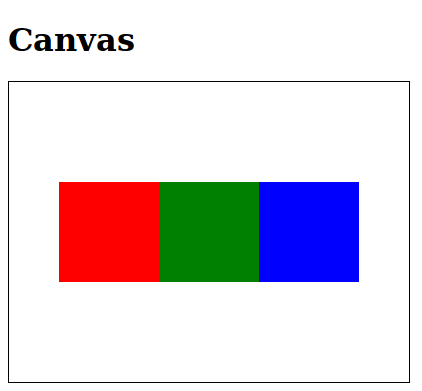
\includegraphics[width=0.7\textwidth]{canvas_ex.png}
\caption{Tre rettangoli disegnati nel canvas}
\label{label:canvasex}
\end{figure}
\clearpage

\section{WebGL: il 3d (realmente) nel web}
Le prime sperimentazioni di un context 3D per l'elemento canvas iniziano nel 2006 all'interno dei laboratori Mozilla ad opera di Vladimir Vukićević\footnote{Corso su WebGL. In \textit{HTML5Today}. Retrieved 12:10, August 14, 2011 from \url{http://www.html5today.it/tutorial/corso-webgl--introduzione}}. Qualche anno più tardi, nel 2009, visto l'interesse suscitato fu istituito il WebGL Working Group. Ad oggi è uno standard cross-platform, cross-browser e royalty-free gestito dal consorzio Khronos Group, responsabile anche di altre importanti tecnologie in campo 3d quale, ad esempio, OpenGL. Nel Marzo 2011 è stata rilasciata la versione 1.0 della specifica\footnote{WebGL Specification. In \textit{Khronos Group}. Retrieved 9:20, July 29, 2011 from \url{https://www.khronos.org/registry/webgl/specs/1.0/}}.

WebGL, acronimo di Web-based Graphics Library, è un'interfaccia di programmazione che consente di creare e gestire contenuti 3d all'interno della pagina web. Per mezzo del tag \texttt{<canvas>} espone una DOM API di basso livello, utilizzabile, dunque, attraverso qualsiasi linguaggio ``DOM-compatibile'' (vedi Javascript, Java). Queste caratteristiche consentono di mettere da parte i plugin di terze parti (spesso soluzioni proprietarie) e di accedere ad un 3d "nativo" del web. Un browser WebGL compatibile si occuperà di fornire l'accelerazione grafica sfruttando l'hardware presente sulla macchina, interfacciandosi direttamente con i driver, con risultati performanti di alta qualità.

Non a caso infatti WebGL poggia su due tecnologie, consolidate e ampiamente diffuse, quali OpenGL ES2, API per la grafica 2D e 3D in sistemi embedded (console, telefono, veicoli, etc...), e l'OpenGL Shading Language (GLSL) per la creazione di ``Shader''\footnote{Gli shader sono insiemi di istruzioni, altamente flessibili e riutilizzabili, che definiscono in ogni parte l'aspetto finale che l'oggetto avrà dopo la fase di rendering.}. L'utilizzo di queste tecnolgie fa di WebGL un'interfaccia di basso livello e sebbene da una parte questo porti enormi benefici sul piano dell'efficienza e della qualità, dall'altra si introduce un'alto livello complessità, anche per la gestione di contenuti semplicissimi come quelli in Figura ~\ref{label:spinwebgl}: \textit{``WebGL is a low-level API, so it's not for the faint of heart. OpenGL's shading language, GLSL, is itself an entire programming environment. As a result, even simple things in WebGL take quite a bit of code. You have to load, compile, and link shaders, set up the variables to be passed in to the shaders, and also perform matrix math to animate shapes.''}. Il bagaglio di conoscenze richieste per utilizzare questa tecnologia è enorme come lo sono, di certo, lo sforzo e il tempo richiesti per apprenderle, malgrado questo sia poi il compito di uno sviluppatore.

\begin{figure}[Ht]
\centering
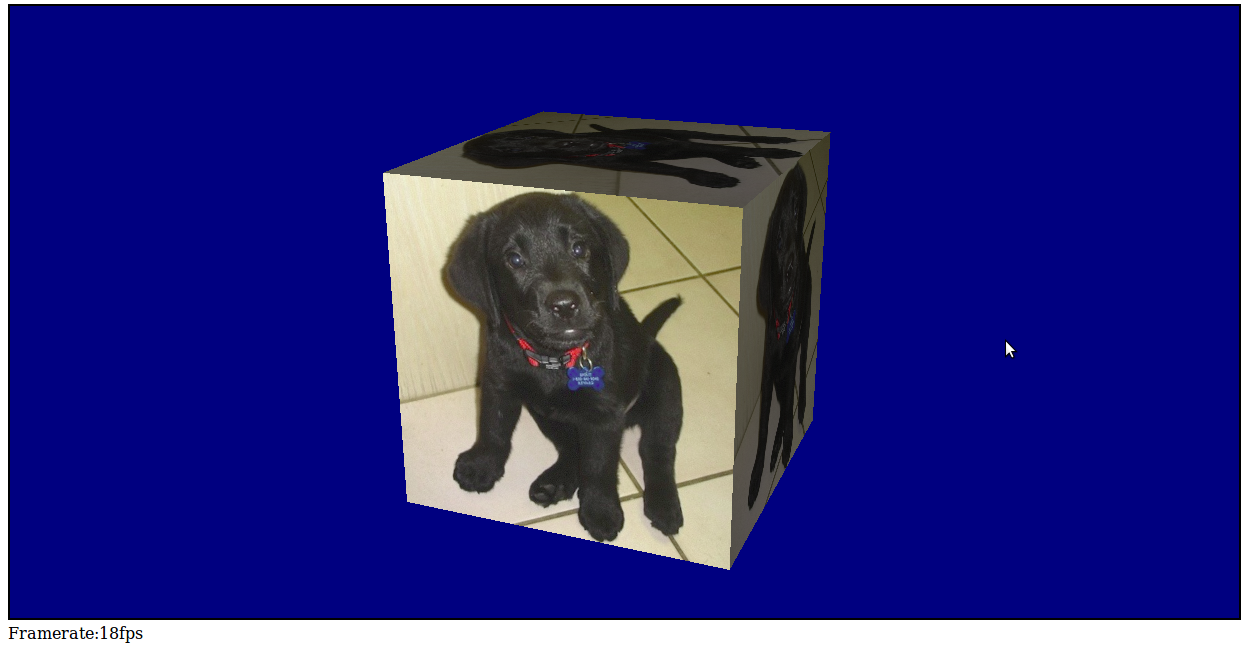
\includegraphics[width=0.7\textwidth]{spinning_webgl.png}
\caption{Cubo con texture in un canvas renderizzato con WebGL}
\label{label:spinwebgl}
\end{figure}

In conclusione WebGL non è uno strumento ``ready-to-use'' e questo potrebbe non giocare a suo favore. Tuttavia, stanno già nascendo librerie di più alto livello che fungono da ``wrapper'' e agevolano la vita al programmatore\footnote{GLGE Official Website. In \textit{GLGE}. Retrieved 7:22, August 18, 2011 from http://www.glge.org/}, mascherando la complessa natura di WebGL e consentendogli dunque di concentrarsi pienamente sulla creazione di contenuti per web. Tra queste vi è sicuramente X3DOM, un framework che tenta di unire il vecchio X3D, consolidata tecnologia di ieri, senza dubbio ``user-friendly'', con il giovane e complicato WebGL.


\section{X3DOM}
Quanto visto finora con WebgGL consente di introdurre e gestire elementi di grafica 3d nel contesto web utilizzado un paradigma di programmazione imperativo. Ciò che manca è un modo semplice per integrare in maniera dichiarativa contenuti 3d all'interno del DOM di una pagina HTML. E' proprio quello che il framework X3DOM cerca di fare, recuperando un percorso già iniziato dall'X3D Working Group per una piena integrazione di X3D con HTML5. L'obiettivo finale è quello di incorporare una scena X3D all'interno del DOM, come già avvenuto per SVG, consentendone la manipolazione semplicemente interagendo con i nodi stessi e grazie al supporto degli eventi HTML per i nodi stessi.

Oltre però ad integrare X3D e HTML5 e necessario poi renderizzare in qualche modo questi contenuti per renderli visibili all'utente finale. Il framework opensource X3DOM 

X3DOM è un framework sperimentale ed open source il cui scopo è quello di cercare di integrare l'HTML5 con contenuti 3D dichiarativi. 
La linea seguita durante lo sviluppo è quella di soddisfare le correnti specifiche dell'HTML5 riguardo i contenuti 3D dichiarativi\cite{W3C-d} e 
permettere l'inclusione di elementi X3D come parte di un qualsiasi albero DOM HTML5. X3DOM è basato principalmente su due tecnologie: X3D e HTML5.
La scelta dell'utilizzo dell'X3D come modello per lo scene-graph si fonda principalmente su tre motivazioni:
\begin{enumerate}
	\item X3D è uno standard ISO maturo e consolidato, che già definisce la codifica XML.
	\item Le specifiche HTML5 già fanno un uso esplicito dell'X3D per scene 3D dichiarative, anche se stanno in una singola riga:
		\\*
		\begin{tabular}{l}
		\bfseries 13.2 Declarative 3D scenes\\*
		\textit{Embedding 3D imagery into XHTML documents is the domain} \\*
		\textit{of X3D, or technologies based on X3D that are namespace-aware.}\\*
		Non specificano però come l'integrazione dovrebbe avvenire\\*
		e cosa più importante, come accedere ai contenuti dello scene-graph.\\*
		\end{tabular}
	\item Esiste già un'interfaccia al DOM tree descritta nel X3D-Programming Language Binding Interface \cite{Web3DConsortium-c}. Come per il punto precedente 
			manca un meccanismo di aggiornamento live dei contenuti dell'albero DOM.
\end{enumerate}
Per lo stesso motivo, l'HTML5 viene utilizzato poiché già utilizza l'X3D per scene 3D dichiarative. Tuttavia, come già detto precedentemente, 
l'HTML5 non specifica come integrare e accedere ai contenuti dello scene-graph. L'intento è quello di estendere il modello di per produrre delle 
immagini in place, piuttosto che all'interno di un plugin aggiuntivo. I nodi X3D sono direttamente integrati con gli elementi DOM e il sottosistema
X3D viene principalmente utilizzato per effettuare un render della scena. L'intera manipolazione dello scene-graph avviene servendosi delle interfacce 
di scripting di un qualsiasi browser standard basato su DOM, come in un tradizionale documento DHTML.
Nei paragrafi successivi verranno trattate le componenti principali dell'architettura alla base delll'X3DOM, mostrata anche in figura.

\clearpage
\subsection{Connettore}
Il connettore è il cuore di questa architettura. Consente di connette il frontends del browser con il backends 
dell'X3D e supporta dei meccanismi per comunicare i cambiamenti nella rappresentazione DOM o in quella X3D. 
L'architettura non usa direttamente l'albero DOM per il rendering della scena ma crea un albero X3D sincronizzato con l'altro. 
Il connettore include anche un DOM/X3D adapter per supportare differenti backends e frontends. Gli sviluppatori hanno previsto 
la presenza di almeno due frontends adapter per Firefox e WebKit e due backends adapter per differenti X3D runtimes (Instant Reality, FreeX3D). 
La corrente implementazione di X3DOM è basata sulle WebGl, mentre beckends alternativi come plugins X3D già esistenti o Flash saranno implementati 
successivamente. Nella figura è mostrato il corrente stato di sviluppo del progetto. Il frontends adapter deve essere in grado 
di accedere direttamente al contenuto dell'albero DOM. Non dovrebbe leggere e analizzare un XML-data-stream, ma leggere e scrivere la 
rappresentazione del DOM. Di conseguenza il backends adapter ha accesso diretto al contesto X3D runtime che include la scena X3D, la quale 
riflette l'albero DOM. Il compito principale del connettore è mantenere entrambe le rappresentazioni sincronizzate e distribuire i 
cambiamenti in entrambe le direzioni.
 
\subsection{Model Update}
Qualsiasi aggiornamento sull'albero DOM, come la creazione, la modifica e la rimozione di elementi DOM, deve riflettersi sull'albero X3D, 
usando il backends adapter. Ciò implica che gli elementi DOM rappresentano direttamente nodi X3D, ma anche strutture addizionali 
come le Route X3D.

\subsection{ObserverResponse}
A seconda del profilo supportato il modello in esecuzione (execution-model) può creare dei cambiamenti nell'albero X3D 
in base al tempo o all'azione dell'utente. Il connettore deve essere in grado di distribuire questi cambiamenti indietro 
nella rappresentazione DOM. Questo sarà reso possibile connettendo l'Observer con specifici elementi dell'albero X3D che 
distribuiranno questi cambiamenti.

\section{Innovazione introdotta da X3DOM}
\subsection{Assenza di plugin}
I sistemi basati su plugin hanno due grandi inconvenienti. Primo, i plugins non sono installati di default sulla 
maggior parte dei sistemi. Di conseguenza, l'utente si deve occupare dell'installazione del plugin e dei problemi di sicurezza e di 
incompatibilità con il browser o il sistema operativo. In secondo luogo, questo tipo di sistemi definisce un'applicazione ed un modello 
di eventi all'interno del plugin che è disaccoppiato dal contenuto DOM della pagina web.
\subsection{Programmazione dichiarativa}
Grazie all'HTML5 esistono già tecnologie per la visualizzazione di scene 3D come canvas3D. Tuttavia quest'ultima è un'interfaccia di 
basso livello, dove il programmatore JavaScript deve manipolare direttamente matrici 4x4, al contrario di quello che avviene utilizzando 
l'X3D per la descrizione di scene 3D.
\subsection{DOM}
La modifica di un nodo all'interno dello scene-graph è molto semplice: al nodo si accede infatti come ad un qualsiasi nodo del 
DOM del browser. Esempio:\\
Codice HTML/X3D:
\lstset{language=HTML}
\begin{lstlisting}
[...]
<group id="root"></group>
[...]
\end{lstlisting}
HTML-Script per l'aggiunta di un nodo:
\begin{lstlisting}[language=Java]
root = document.getElementByid("id");
trans = document.createElement('Transform');
trans.setAttribute("translation", "1 2 3" );
root.appendChild(trans);
\end{lstlisting}
HTML-Script per la rimozione di un nodo:
\begin{lstlisting}[language=Java]
document.getElementById("root").removeChild(trans);
\end{lstlisting}
